The instruments used to conduct spallation experiments are comprised of various different components that are used to alter the beam of neutrons and/or to measure/detect certain phenomena. Such components include neutron detectors, which capture the pulse of energy after going through a target, and disk choppers, which interrupt the beam so that only neutrons of a certain speed may reach the material that we wish to study. Precise knowledge of the properties and whereabouts of these components is vital in order to analyse the results of our experiments reliably. 

NeXus is an effort by an international group of scientists to define a common data exchange and archival format for neutron, X-ray and muon experiments. NeXus is built on top of the scientific data format HDF5 and adds domain-specific rules for organizing data within HDF5 files.

\begin{figure}
\caption{A typical nexus file layout with shape definition}
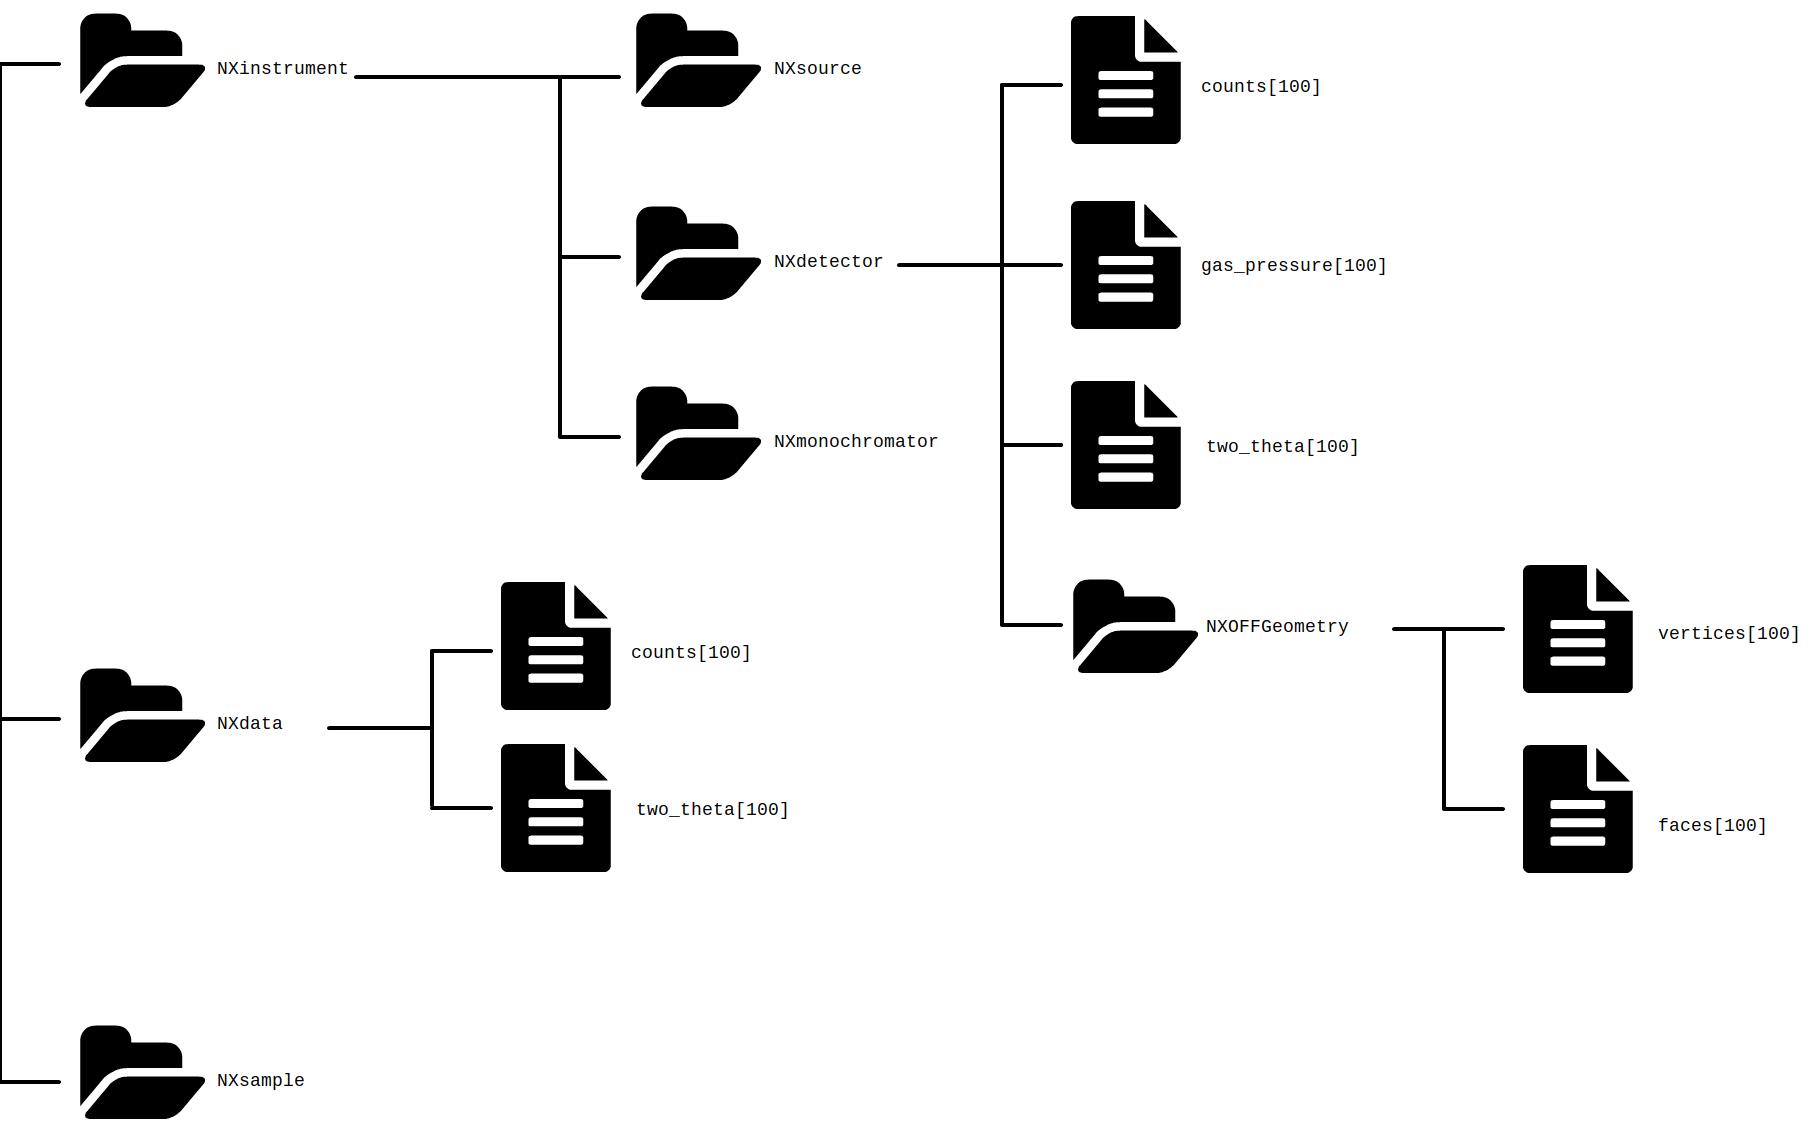
\includegraphics[width=\linewidth]{nexusdiagram.png}
\end{figure}

A recent addition to the NeXus standard means components that are used in experiments can specify shape definition to describe their placement, size and geometry. Transformations (NXtransformations) can be applied to these components when their position changes during or before the experiment. 
